% scenarios2.tex
% --
% James Jackson <eeu203@bangor.ac.uk>



% We want this to be an article
\documentclass[pdftex,a4paper,10pt,titlepage]{article}

% Outline the packages to be used (natbib, fancyhdr, url, geometry, hyperref)
\usepackage[utf8]{inputenc}
\usepackage[round,authoryear,sort]{natbib}
\usepackage{fancyhdr}
\usepackage[margin=0.5in]{geometry}
\usepackage[hidelinks]{hyperref}
\usepackage[anythingbreaks]{breakurl}
\usepackage{graphicx}
\usepackage{hyperref}
\usepackage{amsmath}
\usepackage[T1]{fontenc}
\usepackage{inconsolata}

\usepackage{color}

\definecolor{pblue}{rgb}{0.13,0.13,1}
\definecolor{pgreen}{rgb}{0,0.5,0}
\definecolor{pred}{rgb}{0.9,0,0}
\definecolor{pgrey}{rgb}{0.46,0.45,0.48}

\usepackage{listings}
\lstset{language=Java,
  showspaces=false,
  showtabs=false,
  breaklines=true,
  showstringspaces=false,
  breakatwhitespace=true,
  commentstyle=\color{pgreen},
  keywordstyle=\color{pblue},
  stringstyle=\color{pred},
  basicstyle=\ttfamily,
  moredelim=[il][\textcolor{pgrey}]{$$},
  moredelim=[is][\textcolor{pgrey}]{\%\%}{\%\%}
}

\graphicspath{ {.} }



\setcounter{secnumdepth}{4}


% Begin the document
\begin{document}



% Define title and make it (this will include the date by default
\title{\textbf{ICP-2027 / Data Structures \& Algorithms} \\ Assessment 2\\ Comparative Studies of BST and Sorted Arrays}
\author{
James Jackson \\ \texttt{<eeu203@bangor.ac.uk>}
}
\maketitle



% Begin the abstract, defining what this article is about.
%\begin{abstract}
%abstract
%\end{abstract}

% Render stuff which isn't top matter on a separate page
\pagebreak




% Set up page style for fancy headers, along with the header information (and page width!)
\newgeometry{margin=1.0in}
\pagestyle{fancy}
\fancyhf{}
\lhead{James Jackson \texttt{(eeu203)}}
\rhead{ICP-2027}
\cfoot{\thepage}

\tableofcontents

\pagebreak

\section{Introduction}
In this assessment, one will have an experience of empirically comparing Binary Search Trees and
Sorted Arrays with their associated algorithms.

Javascript will be used to run studies on the length of a search on data within binary search trees (BST) and binary search over a sorted array.

Using Javascript necessitates the full implementation of a BST as well as a binary search function. The decision has been made to avoid recursion for implementations to ensure that the program does not use unnecessary space and computation as well as ensuring that it works regardless of the JS interpreter stack space for a given browser. 

\section{Definitions}

\subsection{Binary Search Tree (BST)}
A BST is that which each node contains it’s given element as well as a link to a node containing an element of lesser value and a link to a node containing an element of greater value. The first element to be added to a BST is put in the root position and will act as the entry point to the tree. 

In order to allow for a more well balanced tree (nodes evenly spread on either side) it will be necessary to ensure that data entered into the tree is not sequential. Entering sequential data into a tree would make for an ill-balanced tree as each new node would be added to either the greater (or lesser depending on the sequence) point at each insertion, this would cause a search function to have to iterate over the entire tree giving it a time complexity of $O(n)$. With non-sequential data it is possible for a search to have a complexity of $O(\log{}n)$ as each iteration of the search can “cut off” on half of the tree (having the problem).

For this study the BST will be simplified to include only a few required functions, namely:
\subsubsection{function add(value)}
Adds a new node to the tree with the supplied value.
Algorithm (Pseudocode):
\begin{lstlisting}[language=java]
if(root node is null){
  set root node to be new node with value
} else {
  set pointer variable to point to root
  while(){
    if(value < pointer value){
      if(pointer left node is null){
        set pointer left to be new node with value
        break loop
      } else {
        set pointer to be pointer left
      } else if (value > pointer value)
        if(pointer right node is null){
          set pointer right to be new node with value
          break loop
        } else {
          set pointer to be pointer right
        }
      } else node exists {
        break loop 
      }
  }
}
\end{lstlisting}

\pagebreak

\subsubsection{function contains(value)}
Returns a value greater than 0 if the value is stored in the tree, the return value represents the length of the path to the node (i.e. the number of nodes compared to reach that point).
Algorithm (Pseudocode):
\begin{lstlisting}[language=java]
count = 0
while(pointer is not null){
  if(value < pointer value){
    set pointer to pointer left
    count ++
  } else if (value > pointer value){
    set pointer to pointer right
    count ++
  } else {
    return count; 
  } 
}
return 0
\end{lstlisting}

Because this is an implementation intended solely for the purpose of this study, it will be assumed that each node will only hold integer values, for comparisons in both adding nodes and finding. A node is simply a javascript object of the following definition.
\begin{lstlisting}[language=java]
node = { data, left, right }
\end{lstlisting}

\subsection{Binary Search}
There two fundamental rules to ensure the success of a binary search and therefore allow a time complexity of $O(\log{}n)$
\begin{itemize}
\item The data structure must allow immediate access to the middle member: anything less than immediate will lead to iteration over each member leading, in turn, to time complexities of $O(n)$.
\item The data structure must be sorted: assumptions need to be made about the nature of neighbouring members to allow the search to work i.e. any member element in a lower index is of a lower value and any member element in a greater index is of a greater value.

\end{itemize}

Algorithm (Pseudocode):
\begin{lstlisting}[language=java]
start = 0
end = array length - 1
count = 0
while (start <= end){
  count ++
  middle = (start + end) / 2
  current = array[middle]
  if(value > current){
    start = middle + 1
  } else if (value < current) {
    end = middle - 1
  } else {
    return count
  }
}
return -1 
\end{lstlisting}
\pagebreak
The calculation $(start + end) / 2$ would need to be floored to ensure an integer value is returned, this can be done in one of three ways.

\begin{itemize}
\item \begin{lstlisting}[language=java] 
Math.floor((start + end) / 2); // floating point division and invocation of Math class. 
\end{lstlisting}

\item \begin{lstlisting}[language=java] 
(start + end) / 2 | 0; // floating point division and bitwise or 0 to drop the decimal.
\end{lstlisting}

\item \begin{lstlisting}[language=java] 
(start + end) >> 1 | 0; // bitwise right shift the value to half and and bitwise or 0 to drop the decimal. floating point division is not used therefore making this approach computationally cheaper.
\end{lstlisting}
\end{itemize}

The time complexity of a binary search on a sorted array is $O(\log{}n)$ as at each point the algorithm removes one half of the remaining elements after the comparison to the middle element. This can be outlined by the following table (linear search for comparison).

\begin{center}
    \begin{tabular}{ | l | l | l  |}
\hline
    & \multicolumn{2}{ | c |}{Maximum Comparisons} \\
  
    \hline
    \textbf{Array Length} & \textbf{Binary Search} & \textbf{Linear Search}  \\  \hline
    10 & 3 & 10  \\ \hline
    1000 & 10 & 1000 \\ \hline
    100000 & 17 & 100000 \\ \hline
    1000000 & 20 & 1000000  \\
    \hline
    \end{tabular}
\end{center}

\section{Expected Results}
\subsection{Binary Search Tree}
The time complexity of searching over a BST is $O(\log{}n)$ when the tree is well balanced, i.e. the data is evenly distributed across the tree and the tree has $\log{}n$ levels to traverse. This is the best case. A very ill balanced tree search has a time complexity of $O(n)$. I this study a shuffled array will be added to the tree. As the array is to be shuffled it is highly unlikely, although not completely impossible, that the tree will be severely ill balanced. It is conversely unlikely that the data will be completely evenly distributed. The expectation is that the search plot will follow a curve similar to $y = \log{}x$ but will be above this value for each array size. Also, due to fluctuating tree depth, it is likely that the search lengths will vary in value when compared to that of the sorted array.
\subsection{Binary Search}
As, by definition, the data in the array is in sequence it is only possible to split the array $\log{}n$ times making a Binary Search time complexity $O(\log{}n)$ at worst. It is expected that the curve of lengths of searches for binary search will be below the $y = \log{}x$ as the length is more likely to finish prior to reaching the end of the algorithm.


%\pagebreak
\section{Implementation}
Algorithm (Pseudocode)
\begin{lstlisting}[language=java]
comparisonsArray[][]
for(i: 100 to 10000){
  create array length i;
  fill array 0 to i - 1
  // ----- start BST test only
  shuffle array
  fill new BST with array
  // ----- end BST test only
  comparisons = 0
  for(j: 0 to 1000){
    comparisons += find(array[random index]);
  }
  push [i, comparisons/1000] onto comparisonsArray;
}
 
\end{lstlisting}

\subsection{Binary Search Tree}
\begin{lstlisting}[language=java,frame=single]
/**
 * Binary Search Tree implementation, limited to two functions
 * add(data) and contains(data), tree is intiated with no nodes
 */
function BST(){
  this.root = null;

  /**
   * add function adds a new node in a tree in the correct place
   * will not add if the data already exists.
   */
  this.add = function(data){
    var newNode = new BST_Node(data);
    var pointer;
    // if root is null we need to add a new node at that point
    if (this.root === null){
      this.root = newNode;
    } else {
      pointer = this.root;
      while(true){
        if (data < pointer.data){
          if (pointer.left === null){
            pointer.left = newNode;
            break;
          } else {
            pointer = pointer.left;
          }
        } else if (data > pointer.data){
          if (pointer.right === null){
            pointer.right = newNode;
            break;
          } else {
            pointer = pointer.right;
          }
        // data already present in tree
        } else {
            break;
        }
      }
    }
  };

  /**
   * contains function searches the tree for given data and returns
   * the length of the search if successful or 0 if unsuccessfull
   */
  this.contains = function(data){
    var comps = 0;
    var pointer = this.root;
    while(pointer){
      if(data < pointer.data){
        pointer = pointer.left;
        comps++;
      } else if(data > pointer.data){
        pointer = pointer.right;
        comps++;
      } else {
        return comps;
      }
    }
    return 0;
  };
}

/**
 * Implementation of a binary search tree node
 */
function BST_Node(nodeData){
  this.left = null;
  this.right = null;
  this.data = nodeData;
}
\end{lstlisting}

\subsection{Binary Search}
\begin{lstlisting}[language=java,frame=single]
/**
 * binarySearch, searches a given array to find a given element
 */
function binarySearch(array, find){
  var start = 0;
  var end = array.length - 1;
  var mid = 0;
  var currentElem;
  var comps = 0;


  while(start <= end){
    comps++;
    mid = (start + end) >> 1;
    currentElem = array[mid];
    if(find > currentElem)
      start = mid + 1;
    else if(find < currentElem)
      end = mid - 1;
    else
      return comps;
  }
  return -1;
}
\end{lstlisting}

\pagebreak
\section{Results \& Conclusions}

The tests can be run from here \url{http://jamesjacko.github.io/bst-js/} \footnote{Binary search test takes up to 20 seconds while the BST can take a few minutes (i/o is kept to a minimum during execution and browser compatible Javascript does not support multi threading, hence the lack of progress feedback).}
\begin{figure}
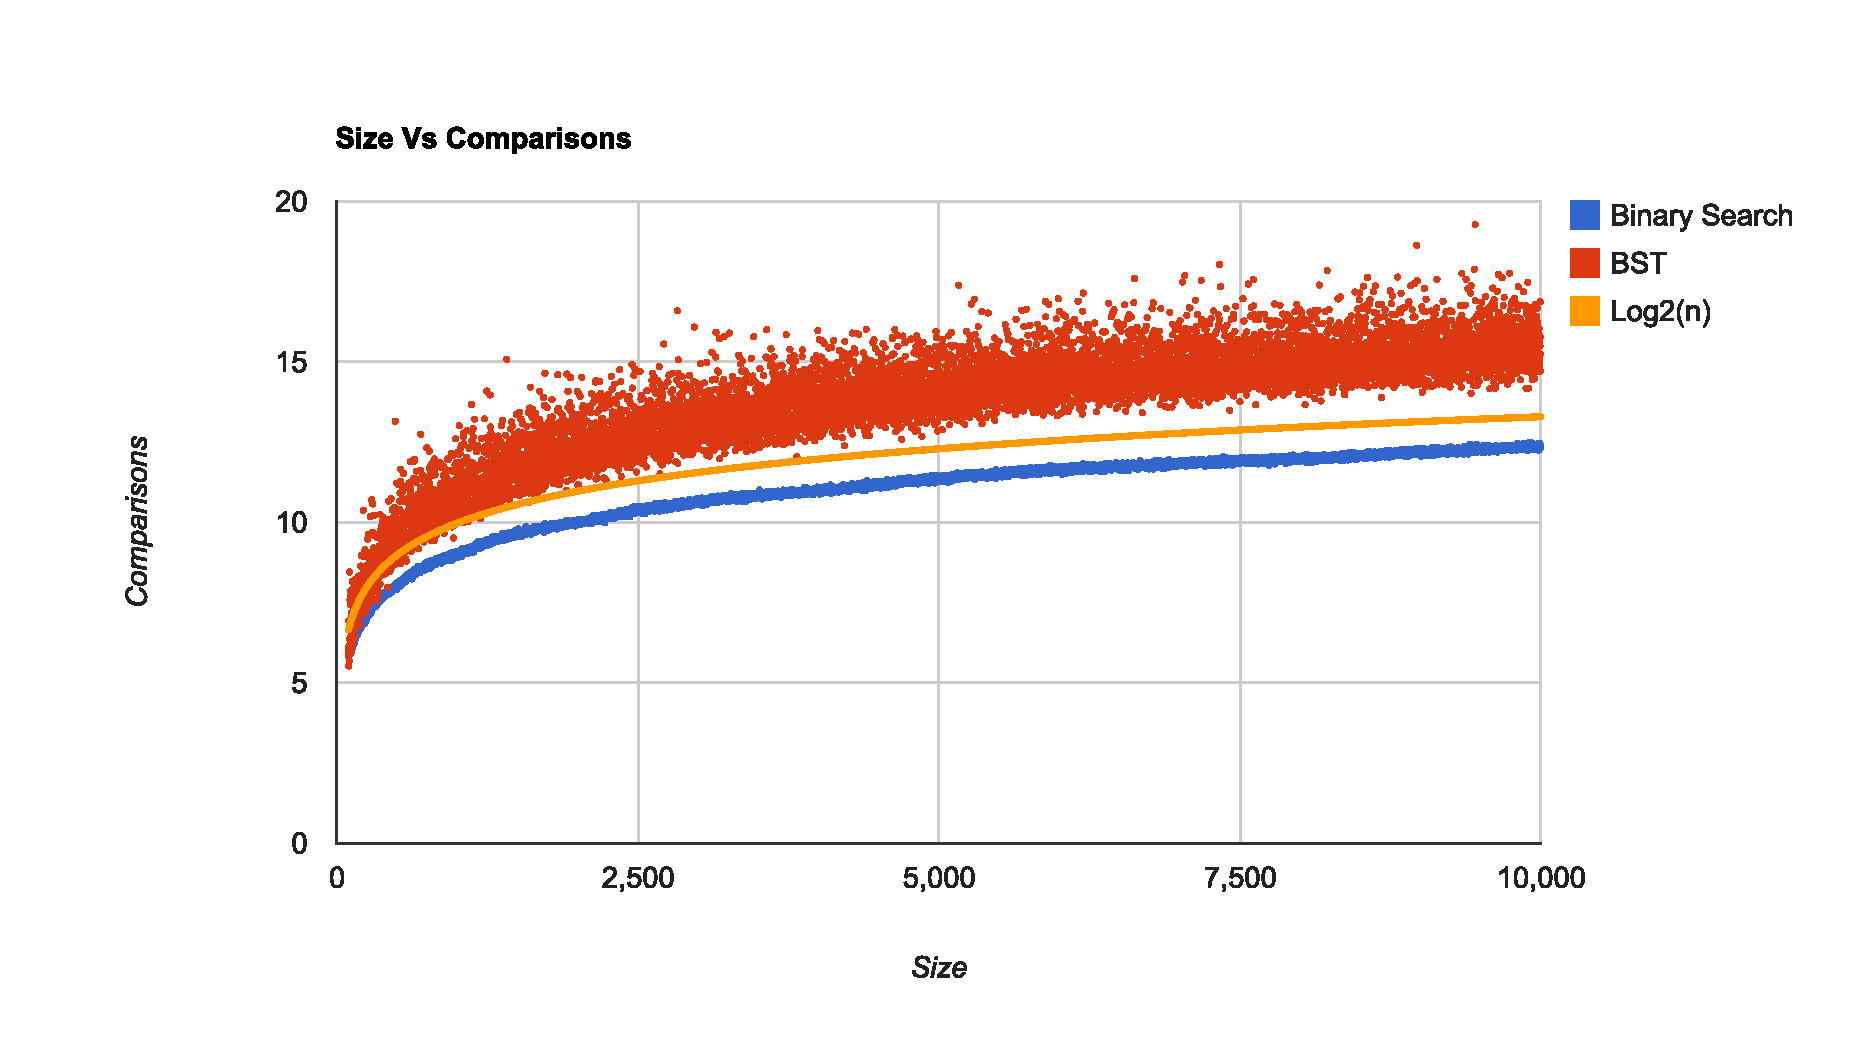
\includegraphics[width=\textwidth]{chart}
\caption{Each point represents average of the 1000 tests, $y = \log{2}(x)$ curve for comparison}
\label{fig:Study Output}
\end{figure}

In both cases the results follow the pattern of a $y = \log{2}(x)$ curve allowing the deduction that both are functioning on or around a $O(\log{}n)$ time complexity, where there is variation is in the initial state of the data. 
\subsection{Binary Search}
In test run on the binary search function the data is always sequential (a constraint defined in the original algorithm) it is merely the element to be found which is picked at random, this allows the function to maintain a time complexity of $O(\log{}n)$ at worst i.e. maximum number of comparisons needed. 
\subsection{Binary Search Tree}
In the case of the BST, the tree is populated at random meaning that there is no guarantee how balanced the tree is, in some cases it could be very well balanced in other cases more ill balanced making the number of comparisons more sporadic than that of the binary search. As noted above there is still a trend to a log curve although it is not quite $\log{2}(n)$. 

\subsection{Conclusion}
When comparing search efficiency on both the BST and Binary search, the conclusion, dictated by the plot, is that a Binary search on a sorted array is more efficient as it is consistently at or below $O(\log{}n)$, a BST fluctuates at just above $O(\log{}n)$. This conclusion is very limited to the initial state of the data in both cases. If the data is not sorted binary search is simply not possible, if a BST is filled with sequential data the tree will be ill balanced and searching will have time complexity of $O(n)$. 
\pagebreak
\subsection{Recommendations}
Decisions on which is more suitable to a given application must be made on the state of the data to be searched. If the data is sorted then using a binary search on an array is a good option. Unsorted data would lend itself better to being searched using a BST as sorting an array for binary search would mean implementation of a sorting algorithm such as mergesort ($O(n\log{}n)$), heapsort ($O(n\log{}n)$) etc.

\subsection{Limitations}

\subsubsection{Sample size}
Given a much bigger sample would allow for further in depth analysis of the two approaches, while Binary Search is effective and consistent it would start to fall down as the array is stretched to it’s inherent memory space limitations, for member numbers in the millions or billions. A study of 100 - 1,000,000,000 would likely yield a different conclusion in terms of feasibility of algorithm use.

\subsubsection{Plot Averaging}
As highlighted each point on the plot is an average of each 1000 tests, it would also be useful to plot the raw data to see the possible fluctuations in the search lengths, this could further cement the superiority (in terms of time complexity) of the Binary Search as it is likely that much higher search lengths are present in the BST, whereas a Binary Search is limited to $O(\log{}n)$

% End the document
\end{document}